\chapter{Lab 8 - Diode Applications}

%%%%%%%%%%%%%%%%%%%%%%%%%%%%%%%%%%%%%%%%%%%%%%%%%%%%%%%%%%%%%%%%%%%%%%%%%%%%%%%%%%%%%%%%%%%%%%%%%%%%%%%
\section{Objective}
%%%%%%%%%%%%%%%%%%%%%%%%%%%%%%%%%%%%%%%%%%%%%%%%%%%%%%%%%%%%%%%%%%%%%%%%%%%%%%%%%%%%%%%%%%%%%%%%%%%%%%%

The objective of this lab is to introduce diodes and a few of their applications. 

%%%%%%%%%%%%%%%%%%%%%%%%%%%%%%%%%%%%%%%%%%%%%%%%%%%%%%%%%%%%%%%%%%%%%%%%%%%%%%%%%%%%%%%%%%%%%%%%%%%%%%%
\section{Materials}
%%%%%%%%%%%%%%%%%%%%%%%%%%%%%%%%%%%%%%%%%%%%%%%%%%%%%%%%%%%%%%%%%%%%%%%%%%%%%%%%%%%%%%%%%%%%%%%%%%%%%%%

\begin{itemize}
	\item Laptop with LTSpice
	\item Analog Discovery
	\item Breadboard
	\item Wiring kit
	\item Lab parts kit
\end{itemize}

%%%%%%%%%%%%%%%%%%%%%%%%%%%%%%%%%%%%%%%%%%%%%%%%%%%%%%%%%%%%%%%%%%%%%%%%%%%%%%%%%%%%%%%%%%%%%%%%%%%%%%%
\section{Introduction}
%%%%%%%%%%%%%%%%%%%%%%%%%%%%%%%%%%%%%%%%%%%%%%%%%%%%%%%%%%%%%%%%%%%%%%%%%%%%%%%%%%%%%%%%%%%%%%%%%%%%%%%

Diodes are a fundamental circuit element whose one-directional current flow has a variety of applications. Diodes can be used as indicators (light emitting diodes (LEDs)), voltage protection elements, and rectification.


%%%%%%%%%%%%%%%%%%%%%%%%%%%%%%%%%%%%%%%%%%%%%%%%%%%%%%%%%%%%%%%%%%%%%%%%%%%%%%%%%%%%%%%%%%%%%%%%%%%%%%%
\subsection{Diode Operation}
%%%%%%%%%%%%%%%%%%%%%%%%%%%%%%%%%%%%%%%%%%%%%%%%%%%%%%%%%%%%%%%%%%%%%%%%%%%%%%%%%%%%%%%%%%%%%%%%%%%%%%%

Each diode has an anode and cathode, \hyperref[fig:idealDiode]{Figure \ref*{fig:idealDiode} (a)}, and conducts current one-way once the voltage across the diode has reached the forward voltage, often called forward bias, $\mathrm{V_F} \approx 0.7 \; \mathrm{V}$. A diode can also conduct current in the opposite direction when the voltage across the diode is negative, often called reverse bias, where the breakdown voltage, $\mathrm{V_{BR}}$, is large, usually -50 V or less. There is often a small current that flows when a diode is reverse bias, but we will neglect that effect for the purposes of this lab. The schematic symbol for an LED is similar, \hyperref[fig:idealDiode]{Figure \ref*{fig:idealDiode} (b)}, but indicates that light is generated when the diode is operating with a forward bias. And the I-V curve for a typical diode, \hyperref[fig:idealDiode]{Figure \ref*{fig:idealDiode} (c)}.

\begin{figure} [h!]
	\centering
		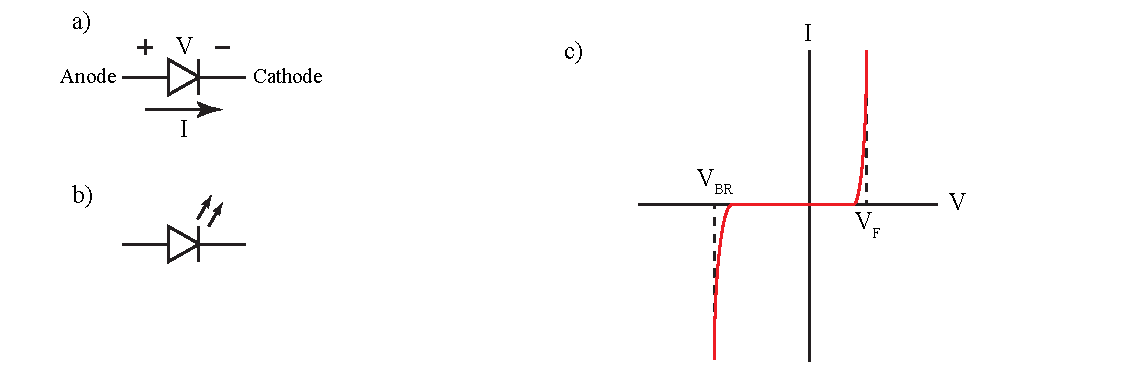
\includegraphics[width=1\textwidth]{Lab6idealDiodes.pdf}
	\caption{Diode schematic symbol with the anode and cathode labeled (a), schematic symbol for an LED (b), and the I-V curve for a diode (c).} \label{fig:idealDiode}
\end{figure}



%%%%%%%%%%%%%%%%%%%%%%%%%%%%%%%%%%%%%%%%%%%%%%%%%%%%%%%%%%%%%%%%%%%%%%%%%%%%%%%%%%%%%%%%%%%%%%%%%%%%%%%
\subsection{Applications}
%%%%%%%%%%%%%%%%%%%%%%%%%%%%%%%%%%%%%%%%%%%%%%%%%%%%%%%%%%%%%%%%%%%%%%%%%%%%%%%%%%%%%%%%%%%%%%%%%%%%%%%

There are a variety of applications for diodes and this lab will focus on only a few, rectifications and clip detection.

%%%%%%%%%%%%%%%%%%%%%%%%%%%%%%%%%%%%%%%%%%%%%%%%%%%%%%%%%%%%%%%%%%%%%%%%%%%%%%%%%%%%%%%%%%%%%%%%%%%%%%%
\subsubsection{Rectifiers}
%%%%%%%%%%%%%%%%%%%%%%%%%%%%%%%%%%%%%%%%%%%%%%%%%%%%%%%%%%%%%%%%%%%%%%%%%%%%%%%%%%%%%%%%%%%%%%%%%%%%%%%

Signal rectification is the process of converting an alternating signal in to its positive or negative components. \hyperref[fig:rect]{Figure \ref*{fig:rect}} is an example of a simple half-wave rectifier. After the input sine wave passes the diodes forward bias voltage, $\approx 0.7$ V, the diode conducts and passes the positive half of the sine wave but doesn't pass the negative half of the sine wave because the diode is reverse bias and does not conduct.

\begin{figure} [h!]
	\centering
		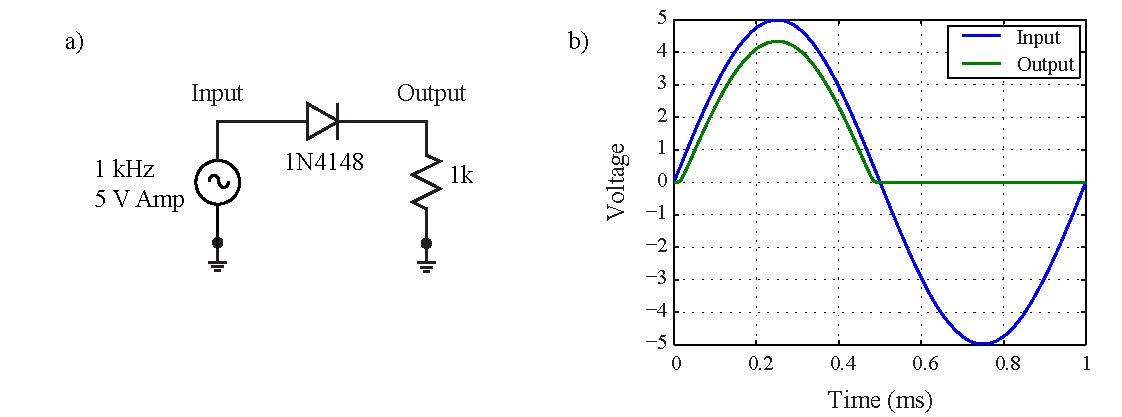
\includegraphics[width=1\textwidth]{Lab6halfrect.pdf}
	\caption{A simple half wave rectifier (a) and the resulting input and output signals (b). } \label{fig:rect}
\end{figure}

Simply adding a capacitor to the half-wave rectifier results in an AC to DC converter, \hyperref[fig:rectWcap]{Figure \ref*{fig:rectWcap}}. The circuit initially behaves as it did previously, once the input sine wave reaches the forward bias voltage, the output follows the input. However, once the sine wave starts to decrease, the output then discharges as a function of an RC time constant, the process then repeats. For higher input frequencies and capacitances, the output cap be approximated as a DC source. 

\begin{figure} [h!]
	\centering
		\includegraphics[width=1\textwidth]{Lab8halfrectWcap.pdf}
	\caption{A simple half wave rectifier but with a capacitor at the output (a) and the resulting input and output signals (b).} \label{fig:rectWcap}
\end{figure}


%%%%%%%%%%%%%%%%%%%%%%%%%%%%%%%%%%%%%%%%%%%%%%%%%%%%%%%%%%%%%%%%%%%%%%%%%%%%%%%%%%%%%%%%%%%%%%%%%%%%%%%
\subsubsection{Clip Detection}
%%%%%%%%%%%%%%%%%%%%%%%%%%%%%%%%%%%%%%%%%%%%%%%%%%%%%%%%%%%%%%%%%%%%%%%%%%%%%%%%%%%%%%%%%%%%%%%%%%%%%%%

There are often cases where the input or output of a system isn't easily accessible for test equipment. A variety of dials, indicators, and display panels are often used to report on the status of a system, examples include current draw, internal voltages, and clip detection. 

Clip detection is the process of determining if a signal is clipping or not. A signal that is clipped, unless desired, can degraded the performance of the system. A clipping detection circuit is able to indicate that the output of the op amp is clipping without viewing the output on an o-scope, but instead through an LED. 

\begin{figure} [h]
	\centering
		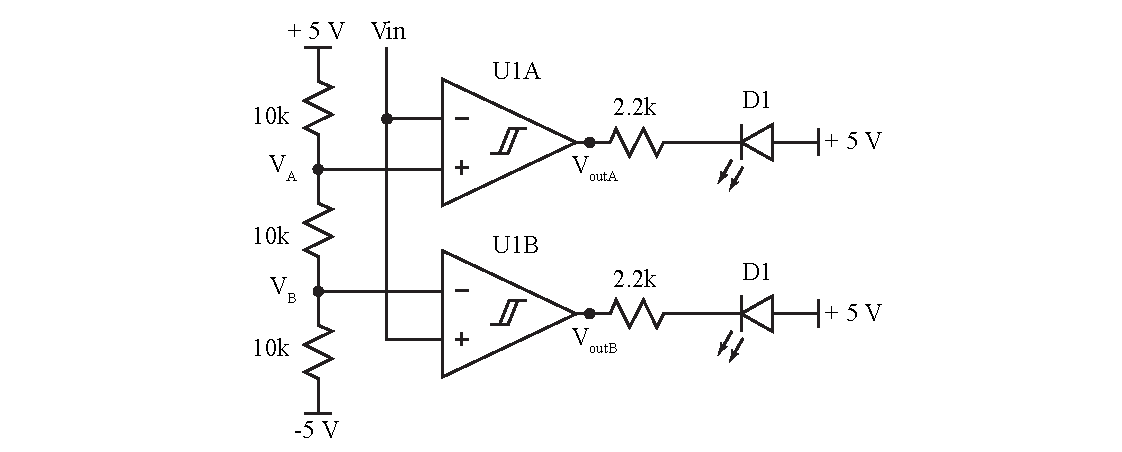
\includegraphics[width=1\textwidth]{Lab6compLED.pdf}
	\caption{A clipping detection circuit. The input is compared to fixed voltages, $V_A$ and $V_B$, by U1A and U1B respectively. If the input voltage is greater, or less, than the reference voltage, the output is pulled low and LED is illuminated.} \label{fig:clipdetect}
\end{figure}

\hyperref[fig:clipdetect]{Figure \ref*{fig:clipdetect}} is an example of a clipping detector. If the input is higher, or lower, than the reference voltage $V_A$, or $V_B$, the LED D1, or D2, illuminates indicated that the input voltage is above, or below, the reference voltage. Note that this circuit does not use op amps, but comparators. Comparators, as the name implies, compares the input at both terminals and produces a digital output, either a 1 (5 V) or 0 (0V), if the positive terminal input is larger than the negative terminal input. 


%%%%%%%%%%%%%%%%%%%%%%%%%%%%%%%%%%%%%%%%%%%%%%%%%%%%%%%%%%%%%%%%%%%%%%%%%%%%%%%%%%%%%%%%%%%%%%%%%%%%%%
\subsection{Potentiometers}
%%%%%%%%%%%%%%%%%%%%%%%%%%%%%%%%%%%%%%%%%%%%%%%%%%%%%%%%%%%%%%%%%%%%%%%%%%%%%%%%%%%%%%%%%%%%%%%%%%%%%%

A potentiometer (or ``pot'') is a three terminal resistor as shown in \hyperref[fig:potcktdia]{Figure \ref*{fig:potcktdia}}. The resistance between terminals 1 and 3 is fixed and is equal to the rated value for the potentiometer. Terminal 2 is connected to a movable contact called the arm or wiper and the resistance between terminals 2 and 1 or between 2 and 3 can be varied by moving the arm. If terminals 1 and 3 are connected across a voltage source, then the voltage between terminals 2 and 1 or between 2 and 3 can be varied by moving the arm. In some cases, terminal 2 is connected to either terminal 1 or 3 so that the resistance from terminals 1 to 3 can be varied. 

\begin{figure}[h] 
	\centering
	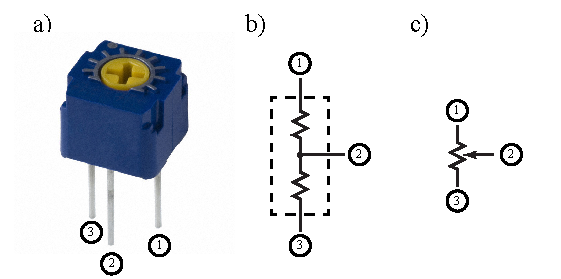
\includegraphics[width=0.5\textwidth]{lab6potdia.pdf}
	\caption{A picture of a practical potentiometer with the appropriate pins labeled (a), an equivalent circuit diagram of a potentiometer with the wiper in a fixed position (b), and the common circuit schematic representation for a potentiometer (c).} \label{fig:potcktdia}
\end{figure}

The potentiometer model in spice is as simple a single resistor, with a resistance equal to the total resistance or less than the total resistance, where the values changes simulation to simulation to the desired resistance. 

%%%%%%%%%%%%%%%%%%%%%%%%%%%%%%%%%%%%%%%%%%%%%%%%%%%%%%%%%%%%%%%%%%%%%%%%%%%%%%%%%%%%%%%%%%%%%%%%%%%%%%%
\section{Big Picture}
%%%%%%%%%%%%%%%%%%%%%%%%%%%%%%%%%%%%%%%%%%%%%%%%%%%%%%%%%%%%%%%%%%%%%%%%%%%%%%%%%%%%%%%%%%%%%%%%%%%%%%%

\begin{figure} [h]
	\centering
		\includegraphics[width=1\textwidth]{Lab8bigpicture.pdf}
	\caption{Big picture with emphasis on the peak detector.} \label{fig:8bp}
\end{figure}

This lab focuses on diode circuits which will help to form the comparator circuits used in the peak detector for the final project. 

%%%%%%%%%%%%%%%%%%%%%%%%%%%%%%%%%%%%%%%%%%%%%%%%%%%%%%%%%%%%%%%%%%%%%%%%%%%%%%%%%%%%%%%%%%%%%%%%%%%%%%%
\section{Pre-Lab Requirements}
%%%%%%%%%%%%%%%%%%%%%%%%%%%%%%%%%%%%%%%%%%%%%%%%%%%%%%%%%%%%%%%%%%%%%%%%%%%%%%%%%%%%%%%%%%%%%%%%%%%%%%%

Complete the following before coming to lab. 

%%%%%%%%%%%%%%%%%%%%%%%%%%%%%%%%%%%%%%%%%%%%%%%%%%%%%%%%%%%%%%%%%%%%%%%%%%%%%%%%%%%%%%%%%%%%%%%%%%%%%%%
\subsection{LTspice Simulations} \label{ssec:6spice}
%%%%%%%%%%%%%%%%%%%%%%%%%%%%%%%%%%%%%%%%%%%%%%%%%%%%%%%%%%%%%%%%%%%%%%%%%%%%%%%%%%%%%%%%%%%%%%%%%%%%%%%

Using LTspice, complete the following.

\begin{enumerate}
	\item Build the circuit in \hyperref[fig:rect]{Figure \ref*{fig:rect} (a)}. Set the input to a 1 kHz, 5 V amplitude sine wave and run a transient simulation with a stop time of 1m (.tran 1m) and plot the input and output.  To use the 1N4148 diode model, right click on the diode after placing it, Pick New Diode, and then choose the 1N4148 model (Mfg. OnSemi). Save an image of the circuit and the plot of the input and output voltage for submission to canvas. \label{itm:8ssec1itm1}
	\item Build the circuit in \hyperref[fig:rectWcap]{Figure \ref*{fig:rectWcap} (a)}. Set the input to a 100 kHz, 5 V amplitude sine wave and run a transient simulation with a stop time of 50u (.tran 50u) and step through possible capacitor values using the following spice directive:
			\begin{verbatim}
			.step param C list 0.001u 0.01u 0.1u 1u
		\end{verbatim}
	 Save an image of the circuit and the plot of the input and output voltage for submission to canvas. \label{itm:8ssec1itm2}
	\item Build the circuit in \hyperref[fig:clipdetect]{Figure \ref*{fig:clipdetect}}. Use the default LED model in LTSpice, and download "slcj016.zip" file from Canvas "Lab Related Files" folder for the LM393 comparator model. Don't use the  "slcj016b.zip" for the comparator model from TI because it's a newer model that doesn't work for input higher than (Vcc-2V). Power the LM393 with +/-5 V. Set the input voltage to a 1 kHz, 5 V amplitude sine wave and run a transient solution with a stop time of 2m (.tran 2m). Plot the input voltage and the current through each diode. Save an image of the circuit and the plot for submission to canvas. \label{itm:8ssec1itm3}
	\item Build the circuit in \hyperref[fig:vga]{Figure \ref*{fig:vga}}. Power the LM393 and TLV272 with  +/-5 V. Set the input voltage to a 1kHz, 0.1 V amplitude sine wave and run a transient solution with a stop time of 2m. Choose the value for R1, 10k pot, so that the diodes conduct current and illuminate. Plot the input voltage, output of the op amp, positive and negative inputs to the comparator, and the current through both LEDs. (6 items total). Save an image of the circuit and the plot for submission to canvas. \label{itm:8ssec1itm4}
\end{enumerate}

\begin{figure}[h] 
	\centering
	\includegraphics[width=1\textwidth]{lab6vga.pdf}
	\caption{A variable gain amplifier, R1 is a potentiometer that can be varied, where the output is checked for clipping.} \label{fig:vga}
\end{figure}


%%%%%%%%%%%%%%%%%%%%%%%%%%%%%%%%%%%%%%%%%%%%%%%%%%%%%%%%%%%%%%%%%%%%%%%%%%%%%%%%%%%%%%%%%%%%%%%%%%%%%%%
\subsection{Breadboard Implementation} \label{ssec:6breadboard}
%%%%%%%%%%%%%%%%%%%%%%%%%%%%%%%%%%%%%%%%%%%%%%%%%%%%%%%%%%%%%%%%%%%%%%%%%%%%%%%%%%%%%%%%%%%%%%%%%%%%%%%

\begin{enumerate}
\item Read the datasheet for the LM393, \url{http://www.ti.com/product/LM393/technicaldocuments}. 
\item Build the circuit in \hyperref[fig:clipdetect]{Figure \ref*{fig:clipdetect}} on a breadboard. It is important to note that the pinout for the comparator chip is the same as the op amp. It works differently, but should be connected the same as the op amp. This means you should still connect pin 8 to +5V and pin 4 to -5V (not GND) just as you have done with the opamp.  Set the input to a 0.5 Hz, 5 V amplitude sine wave. Use the two red LEDS in your lab kit, they're bagged separately. The anode for the LEDs is the longer of the two leads. The diodes will illuminate whenever the input voltage is above or below the reference voltage and should appear to blink in turn. Save the circuit to show your lab instructor at the start of lab. \label{itm:8ssec2itm1}
\end{enumerate}

%%%%%%%%%%%%%%%%%%%%%%%%%%%%%%%%%%%%%%%%%%%%%%%%%%%%%%%%%%%%%%%%%%%%%%%%%%%%%%%%%%%%%%%%%%%%%%%%%%%%%%%
\section{In-Lab Requirements}
%%%%%%%%%%%%%%%%%%%%%%%%%%%%%%%%%%%%%%%%%%%%%%%%%%%%%%%%%%%%%%%%%%%%%%%%%%%%%%%%%%%%%%%%%%%%%%%%%%%%%%%

The following must be completed at the start of lab. 

\begin{enumerate}
	\item \hyperref[ssec:6spice]{Section \ref*{ssec:6spice}}
		\begin{enumerate}
			\item \hyperref[itm:8ssec1itm1]{Item \ref*{itm:8ssec1itm1}}: Half wave rectifier, image of the circuit and the plot of the input and output voltage.
			\item \hyperref[itm:8ssec1itm2]{Item \ref*{itm:8ssec1itm2}}: Half wave rectifier with output smoothing, image of the circuit and the plot of the input and output voltage.
			\item \hyperref[itm:8ssec1itm3]{Item \ref*{itm:8ssec1itm3}}: Clipping circuit, image of the circuit and the plot.
			\item \hyperref[itm:8ssec1itm4]{Item \ref*{itm:8ssec1itm4}}: Variable gain amplifier with clip detector, image of the circuit and the plot.
		\end{enumerate}
	\item \hyperref[ssec:6breadboard]{Section \ref*{ssec:6breadboard}}
		\begin{enumerate}
			\item \hyperref[itm:8ssec1itm5]{Item \ref*{itm:8ssec2itm1}}: Operational clipping circuit. 
		\end{enumerate}
\end{enumerate}

%%%%%%%%%%%%%%%%%%%%%%%%%%%%%%%%%%%%%%%%%%%%%%%%%%%%%%%%%%%%%%%%%%%%%%%%%%%%%%%%%%%%%%%%%%%%%%%%%%%%%%%
\subsection{Breadboard Implementation}
%%%%%%%%%%%%%%%%%%%%%%%%%%%%%%%%%%%%%%%%%%%%%%%%%%%%%%%%%%%%%%%%%%%%%%%%%%%%%%%%%%%%%%%%%%%%%%%%%%%%%%%

\begin{enumerate}
\item Plot the input voltage and the voltage at the output of either comparator, \hyperref[fig:clipdetect]{Figure \ref*{fig:clipdetect}}, on the o-scope and save an image of the display. 
	\item Build the circuit from \hyperref[itm:8ssec1itm1]{Section \ref*{ssec:6spice} - Item \ref*{itm:8ssec1itm1}}. Plot the input and output on the o-scope and save an image of the display.
	\item Build two version of the circuit from \hyperref[itm:8ssec1itm2]{Subsection \ref*{ssec:6spice} - Item \ref*{itm:8ssec1itm2}}, one with where the capacitance is 0.1 uF and the other is 0.01 uF. Plot the outputs of both circuits on the o-scope and save an image of the display. 
	\item Build the circuit from \hyperref[itm:8ssec1itm3]{Subsection \ref*{ssec:6spice} - Item \ref*{itm:8ssec1itm4}}. Set the input to a 0.5 Hz, 0.1 V amplitude sine wave. Vary the potentiometer, increase the gain, so that the LEDs illuminate when the op amp output is greater than the reference voltages. Plot the output of the gain amplifier and the output of either comparator on the o-scope and save an image of the display.
\end{enumerate}


%%%%%%%%%%%%%%%%%%%%%%%%%%%%%%%%%%%%%%%%%%%%%%%%%%%%%%%%%%%%%%%%%%%%%%%%%%%%%%%%%%%%%%%%%%%%%%%%%%%%%%%
\section{Write Up}
%%%%%%%%%%%%%%%%%%%%%%%%%%%%%%%%%%%%%%%%%%%%%%%%%%%%%%%%%%%%%%%%%%%%%%%%%%%%%%%%%%%%%%%%%%%%%%%%%%%%%%%

This write up is different than previous write ups. Instead of comparing ideal and non-ideal values, discuss the operation and limitations of each circuit. For example, the first circuit is limited by forward voltage which limits how much of the signal can be rectified. Backup your discussion with images, all four, from the in-lab portion. Also, include diagrams for each circuit, typically this is not required but for this lab circuit diagrams are required. Do not copy the circuit diagrams from the lab manual, create your own, either digitally or by hand. 




